% A partir del fichero.pdf se genera el fichero a imprimir:
%
% pdfnup --nup 1x2 --paper a4paper --no-landscape filename.pdf
%
\documentclass[handout]{beamer}
\usepackage{ae}
\usepackage[utf8]{inputenc}
\usepackage[american]{babel}
\usepackage{amsmath,amsfonts}
\usepackage{bm}
\mode<presentation>
{
	\usetheme{PaloAlto}
	% or ...
	
	%  \setbeamercovered{transparent}
	% or whatever (possibly just delete it)
	\usecolortheme{dove}
}
\title[Modelos de difusión]{
	MÉTODO DE LOS ELEMENTOS FINITOS. \\
	Modelos de Difusión}
\author[Felipe Gabaldón]{Felipe Gabaldón Castillo}
\date{Madrid, 28 de septiembre de 2017}
\pgfdeclareimage[height=0.5cm]{logo-upm}{upm}
\logo{\pgfuseimage{logo-upm}}

\AtBeginSection[]
{
	\begin{frame}<beamer>
		\frametitle{Índice}
		\tableofcontents[currentsection]
	\end{frame}
}
%%%%%%%%%%%%%%%%%%%%%%%%%%%%%%%%%%%%%%%%%%%%%%%%%%%%%%%%%%%%%%%%%%%%%%%%%%%%%%
\newcommand{\norm}[1]{\lVert #1 \rVert}
\begin{document}
%%%%%%%%%%%%%%%%%%%%%%%%%%%%%%%%%%%%%%%%%%%%%%%%%%%%%%%%%%%%%%%%%%%%%%%%%%%%%%
\begin{frame}
\titlepage
\end{frame}
%%%%%%%%%%%%%%%%%%%%%%%%%%%%%%%%%%%%%%%%%%%%%%%%%%%%%%%%%%%%%%%%%%%%%%%%%%%%%%
\begin{frame}
\frametitle{Índice}
\tableofcontents[pausesections]
\end{frame}
%%%%%%%%%%%%%%%%%%%%%%%%%%%%%%%%%%%%%%%%%%%%%%%%%%%%%%%%%%%%%%%%%%%%%%%%%%%%%%
\section{Introducción}
%%%%%%%%%%%%%%%%%%%%%%%%%%%%%%%%%%%%%%%%%%%%%%%%%%%%%%%%%%%%%%%%%%%%%%%%%%%%%%
\begin{frame}
\frametitle{La ecuación de Poisson}
\parbox{40mm}{
\begin{align*}
\operatorname{div} \bm{q}&=f \textrm{ en }\Omega \\
u&=\overline{u}\textrm{ en } \partial_{u} \Omega \\
\bm{q}\cdot \bm{n}&=q_n \textrm{ en } \partial_{q} \Omega\\
\bm{q}&=-\bm{k} \bm{\nabla}_{x} u
\end{align*}
}
\parbox{50mm}{
\begin{align*}
\mbox{}& \textrm{ (ecuación de balance)} \\
\mbox{}& \textrm{ (condición esencial de contorno)}\\
\mbox{}& \textrm{ (condición natural de contorno)}\\
\mbox{}& \textrm{ (ecuación constitutiva)}
\end{align*}
}
siendo:
\vspace{-5mm}
\begin{align*}
u  &:\textrm{ función potencial (variable básica)} \\
\bm{q}&:\textrm{ vector flujo} \\
f&:\textrm{ fuente} \\
\bm{k}&:\textrm{ tensor constitutivo} \\
\end{align*}
El interés que tiene estudiar aquí la ecuación de Poisson es el
amplio número de modelos físicos que se rigen por esta ecuación, y que
la variable básica es un escalar
\end{frame}
%%%%%%%%%%%%%%%%%%%%%%%%%%%%%%%%%%%%%%%%%%%%%%%%%%%%%%%%%%%%%%%%%%%%%%%%%%%%%%
\begin{frame}
\frametitle{Conducción de calor}
\begin{align*}
\operatorname{div} \bm{q}&=f  \\
\bm{q}&=-\bm{k} \bm{\nabla}_{x} u
\end{align*}
\begin{align*}
u  &:\textrm{\color{red}{Temperatura}} \\
\bm{q}&:\textrm{\color{red}{Flujo de calor por unidad de superficie}} \\
f&:\textrm{\color{red}{Calor generado por unidad de volumen}} \\
\bm{k}&:\textrm{\color{red}{Matriz de conductividades (Ley de Fourier)}}
\end{align*}
\end{frame}
%%%%%%%%%%%%%%%%%%%%%%%%%%%%%%%%%%%%%%%%%%%%%%%%%%%%%%%%%%%%%%%%%%%%%%%%%%%%%%
\begin{frame}
\frametitle{Conducción de calor}
\begin{center}
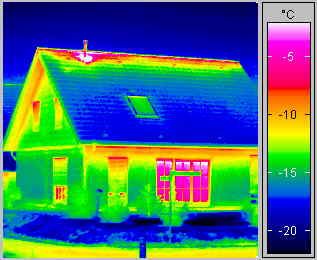
\includegraphics[width=0.65\textwidth]{building_envelope_ir.jpg}
\end{center}
\end{frame}
%%%%%%%%%%%%%%%%%%%%%%%%%%%%%%%%%%%%%%%%%%%%%%%%%%%%%%%%%%%%%%%%%%%%%%%%%%%%%%
\begin{frame}
\frametitle{Flujo en medios porosos}
\begin{align*}
\operatorname{div} \bm{q}&=f  \\
\bm{q}&=-\bm{k} \bm{\nabla}_{x} u
\end{align*}
\begin{align*}
u  &:\textrm{\color{blue}{Altura piezométrica }} (u=\frac{p}{\gamma}+z) \\
\bm{q}&:\textrm{\color{blue}{Velocidad}}\\
f&:\textrm{\color{blue}{Caudal suministrado por unidad de volumen}}\\
\bm{k}&:\textrm{\color{blue}{Matriz de permeabilidades (Ley de Darcy)}}
\end{align*}
\end{frame}
%%%%%%%%%%%%%%%%%%%%%%%%%%%%%%%%%%%%%%%%%%%%%%%%%%%%%%%%%%%%%%%%%%%%%%%%%%%%%%
\begin{frame}
\frametitle{Flujo en medios porosos}
\begin{center}
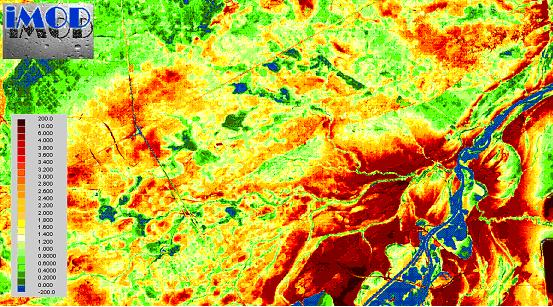
\includegraphics[width=\textwidth]{Deltares_IMOD.jpg}
\end{center}
\end{frame}
%%%%%%%%%%%%%%%%%%%%%%%%%%%%%%%%%%%%%%%%%%%%%%%%%%%%%%%%%%%%%%%%%%%%%%%%%%%%%%
\begin{frame}
\frametitle{Electrostática}
\begin{align*}
\operatorname{div} \bm{q}&=f  \\
\bm{q}&=-\bm{k} \bm{\nabla}_{x} u
\end{align*}
\begin{align*}
u  &:\textrm{\color{green}{Potencial eléctrico}} \\
\bm{q}&:\textrm{\color{green}{Intensidad de campo eléctrico}} \\
f&:\textrm{\color{green}{Carga eléctrica generada por unidad de volumen}} \\
\bm{k}&:\textrm{\color{green}{Matriz de permitividades (Ley de Gauss)}}
\end{align*}
\end{frame}
%%%%%%%%%%%%%%%%%%%%%%%%%%%%%%%%%%%%%%%%%%%%%%%%%%%%%%%%%%%%%%%%%%%%%%%%%%%%%%
\begin{frame}
\frametitle{Electrostática}
\begin{center}
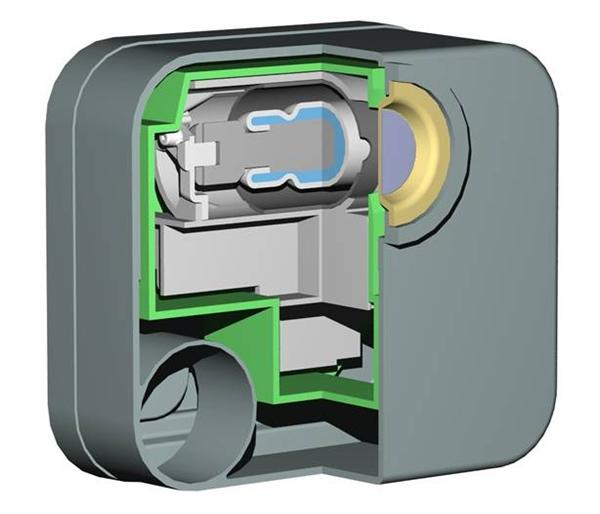
\includegraphics[width=0.4\textwidth]{Model_Geometry_600_514.jpg}
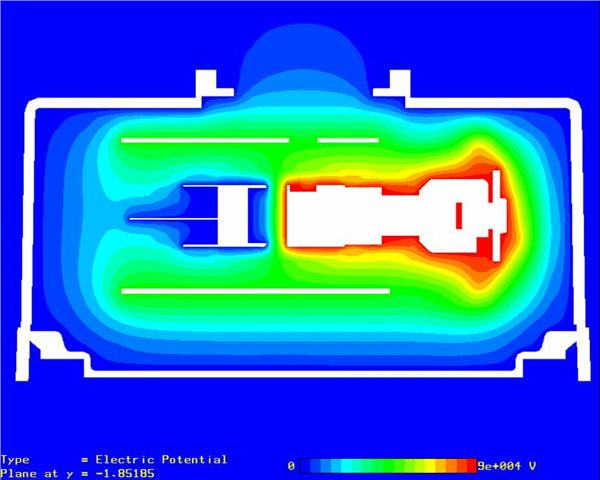
\includegraphics[width=0.6\textwidth]{electric_fields_contour_600_480.jpg}
\end{center}
\end{frame}
%%%%%%%%%%%%%%%%%%%%%%%%%%%%%%%%%%%%%%%%%%%%%%%%%%%%%%%%%%%%%%%%%%%%%%%%%%%%%%
\begin{frame}
\frametitle{Torsión uniforme}
\begin{align*}
\operatorname{div} \bm{q}&=f  \\
\bm{q}&=-\bm{k} \bm{\nabla}_{x} u
\end{align*}
\begin{align*}
u  &:\textrm{\color{magenta}{ Función de tensiones (constante en }} \partial \Omega) \\
\bm{q}&:\textrm{\color{magenta}{ Tensiones tangenciales}} \\
f&: \textrm{ }2 G \theta, \textrm{\color{magenta}{ siendo }} 
\theta \textrm{\color{magenta}{ el giro por unidad de longitud y}} \\
 &\mbox{ }G \textrm{\color{magenta}{ el módulo de cortante}} \\
\sigma_{i3}&= \frac{\partial u}{\partial x_i}, 
\textrm{\color{magenta}{ sería la ecuación constitutiva}}
\end{align*}
\begin{itemize}
\item Otros modelos físicos: flujo irrotacional de fluidos ideales,
lubricación de cojinetes, magnetostática, presiones hidrodinámicas sobre
superficies en movimiento, etc.
\end{itemize}
\end{frame}
%%%%%%%%%%%%%%%%%%%%%%%%%%%%%%%%%%%%%%%%%%%%%%%%%%%%%%%%%%%%%%%%%%%%%%%%%%%%%%
\begin{frame}
\frametitle{Torsión uniforme}
\begin{center}
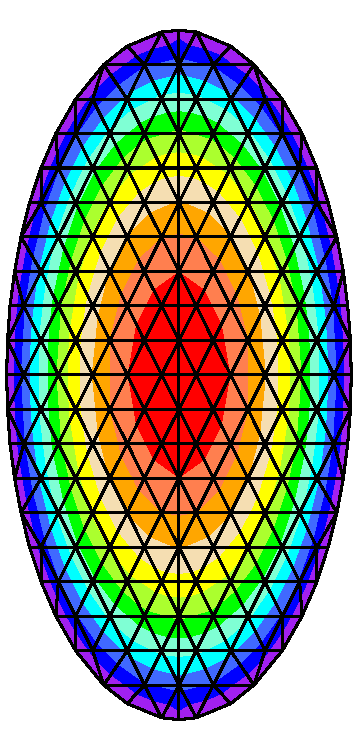
\includegraphics[height=0.95\textheight]{torsion_uni.pdf}
\end{center}
\end{frame}
%%%%%%%%%%%%%%%%%%%%%%%%%%%%%%%%%%%%%%%%%%%%%%%%%%%%%%%%%%%%%%%%%%%%%%%%%%%%%%
\section{Formulación del problema de contorno}
\begin{frame}
\frametitle{Formulación fuerte}

Sea $\overline{\Omega}=\Omega \cup \partial \Omega$ el dominio ocupado
por un medio conductivo ($\overline{\Omega} \subset \mathbb{R}^n$), cuyo
contorno $\partial \Omega$ admite la descomposición
$\partial \Omega=\partial_u \Omega \cup \partial_t \Omega$,
$\partial_u \Omega \cap \partial_t \Omega= \emptyset$. La formulación fuerte
del problema se establece en los siguientes términos:

Dados $f:\Omega \rightarrow \mathbb{R},\quad
\overline{u} :\partial_u \Omega \rightarrow \mathbb{R}, \quad
\overline{q} :\partial_t \Omega \rightarrow \mathbb{R}$, encontrar el
campo de temperaturas $u:\overline{\Omega}\rightarrow \mathbb{R}$ que
cumple:
\begin{align}
\operatorname{div} \bm{q}&=f \textrm{ en } \Omega\\
u&=\overline{u} \textrm{ en } \partial_u \Omega \\
\bm{q}\cdot \bm{n} &=\overline{q} \textrm{ en } \partial_t \Omega
\end{align}
con $\bm{q}=-\bm{k} \bm{\nabla} u$
\end{frame}
%%%%%%%%%%%%%%%%%%%%%%%%%%%%%%%%%%%%%%%%%%%%%%%%%%%%%%%%%%%%%%%%%%%%%%%%%%%%%%
\begin{frame}
\frametitle{Formulación débil}

Dados $f:\Omega \rightarrow \mathbb{R}$ y las funciones
$\overline{u} :\partial_u \Omega \rightarrow \mathbb{R}, \quad
\overline{q} :\partial_t \Omega \rightarrow \mathbb{R}$, encontrar el
campo de temperaturas $u \in \delta \, \mid \, \forall \delta u \in
\nu$ que cumple:
\begin{equation}
\int_{\Omega} 
\left( \bm{q} \cdot \bm{\nabla} \delta u \, + f \delta u \right) \,
d \Omega - \int_{\partial_t \Omega} \overline{q} \delta u \, d \Gamma=0
\end{equation}
siendo:
\begin{align}
\delta&=\left\{
u \in H^1(\Omega,\mathbb{R}) \mid u(\bm{x})=\overline{u}
\; \quad \forall \; \bm{x} \in \partial_u \Omega \right\} \label{trial} \\
{\cal V}&=\left\{
\delta u \in H^1(\Omega,\mathbb{R}) \mid \delta u(\bm{x})=0
\; \quad \forall \; \bm{x} \in \partial_u \Omega \right\} \label{weight}
\end{align}
y $H^1(\Omega,\mathbb{R})$ el espacio de Sobolev de orden $1$ y grado $2$:
$$
H^1=\left\{ u:\Omega \rightarrow \mathbb{R} \quad \mid \quad
\int_{\Omega} \norm{u}_{2,1} \, d\Omega <\infty \right\}
$$
\end{frame}
%%%%%%%%%%%%%%%%%%%%%%%%%%%%%%%%%%%%%%%%%%%%%%%%%%%%%%%%%%%%%%%%%%%%%%%%%%%%%%
\begin{frame}
\frametitle{Equivalencia de las formulaciones fuerte y débil}
\begin{itemize}
\item[1.] $u$ es solución de (S) $\Rightarrow u$ es solución de (W)

Si $u \textrm{ es solución de (S)} \Rightarrow u=\overline{u} \textrm{ en }
\partial_u \Omega \Rightarrow u \in \delta$

Por otra parte:
\begin{align*}
0&= \int_{\Omega} \left( \operatorname{div} \bm{q} -f \right) \delta u \, d \Omega= \\
 &\mbox{ } -\int_{\Omega} \bm{q} \cdot \bm{\nabla} \delta u \, d \Omega+
\int_{\partial \Omega} \bm{q} \cdot \bm{n} \delta u \, d \Gamma -
\int_{\Omega} f \delta u \, d\Omega= \\
 &\mbox{ } - \int_{\Omega} \left(
\bm{q} \cdot \bm{\nabla} \delta u + f \delta u \right) 
d \Omega+
\int_{\partial_t \Omega} \overline{q} \delta u \, d \Gamma
\end{align*}
\end{itemize}
\end{frame}
%%%%%%%%%%%%%%%%%%%%%%%%%%%%%%%%%%%%%%%%%%%%%%%%%%%%%%%%%%%%%%%%%%%%%%%%%%%%%%
\begin{frame}
\frametitle{Equivalencia de las formulaciones fuerte y débil}
\begin{itemize}
\item[2.] $u$ es solución de (W) $\Rightarrow u$ es solución de (S)

Si $u \textrm{ es solución de (W), } u \in \delta \Rightarrow u=g \textrm{ en }
\partial_u \Omega$

Por otra parte, $\forall \delta u \in \nu$ se verifica:
\begin{align}
0&= \int_{\Omega} \bm{q} \cdot \bm{\nabla} \delta u \, d \Omega+
\int_{\Omega} f \delta u \, d\Omega -
\int_{\partial_t \Omega} \overline{q} \delta u \, d \Gamma \nonumber \\
&= \int_{\Omega} \left( -\operatorname{div} \bm{q} +f \right) \delta u \, d \Omega+
\int_{\partial_t \Omega} \left(\bm{q}\cdot \bm{n} - \overline{q}
\right) \delta u \, d \Gamma
\label{auxequi}
\end{align}
con lo que debe demostrarse:
\begin{align*}
\textrm{\color{blue}{a)} }&-\operatorname{div} \bm{q} +f=0 \textrm{ en } \Omega \\
\textrm{\color{blue}{b)} }&\bm{q}\cdot \bm{n} - \overline{q}=0 \textrm{ en } \partial_t \Omega
\end{align*}
\end{itemize}
\end{frame}
%%%%%%%%%%%%%%%%%%%%%%%%%%%%%%%%%%%%%%%%%%%%%%%%%%%%%%%%%%%%%%%%%%%%%%%%%%%%%%
\begin{frame}
\frametitle{Equivalencia de las formulaciones fuerte y débil}
\begin{itemize}
\item[a)] $-\operatorname{div} \bm{q} +f=0 \textrm{ en } \Omega$
\end{itemize}
Sea $\delta u=(-\operatorname{div} \bm{q} +f) \phi$,
donde $\phi$ es una función que verifica:
\begin{align*}
1&) \phi>0 \textrm{ en } \Omega \\
2&) \phi=0 \textrm{ en } \partial \Omega \\
3&) \phi \textrm{ suave }
\end{align*}
Sustituyendo en (\ref{auxequi}):
\begin{align*}
0&=\int_{\Omega} \left(-\operatorname{div} \bm{q} +f \right)^2 \phi \, d\Omega+
\underbrace{\int_{\partial_t \Omega} \phi \left(-\operatorname{div} \bm{q} +f \right)
\left( \bm{q}\cdot \bm{n} - \overline{q} \right) \,d \Gamma}_{=0} \\
&\Rightarrow
-\operatorname{div} \bm{q} +f=0 \textrm{ en } \Omega
\end{align*}
\end{frame}
%%%%%%%%%%%%%%%%%%%%%%%%%%%%%%%%%%%%%%%%%%%%%%%%%%%%%%%%%%%%%%%%%%%%%%%%%%%%%%
\begin{frame}
\frametitle{Equivalencia de las formulaciones fuerte y débil}
\begin{itemize}
\item[b)] $\bm{q}\cdot \bm{n} - \overline{q}=0 \textrm{ en } \partial_t \Omega$
\end{itemize}
Sea ahora $\delta u=(\bm{q}\cdot \bm{n} - \overline{q}) \psi$,
donde $\psi$ verifica:
\begin{align*}
1&) \psi>0 \textrm{ en } \partial_t \Omega \\
2&) \psi=0 \textrm{ en } \partial_u \Omega \\
3&) \psi \textrm{ suave }
\end{align*}
Sustituyendo en (\ref{auxequi}) y teniendo en cuenta que ya se ha demostrado
que $-\operatorname{div} \bm{q} +f=0$ en $\Omega$, resulta:
\begin{equation*}
0=\int_{\partial_t \Omega} \left(\bm{q}\cdot \bm{n} - \overline{q}
\right)^2 \psi \, d \Gamma
\end{equation*}
para lo que debe de verificarse:
\begin{equation*}
\bm{q}\cdot \bm{n} - \overline{q}=0 \textrm{ en } \partial_t \Omega
\end{equation*}
\end{frame}
%%%%%%%%%%%%%%%%%%%%%%%%%%%%%%%%%%%%%%%%%%%%%%%%%%%%%%%%%%%%%%%%%%%%%%%%%%%%%%
\section{Formulación de Galerkin}
\begin{frame}
\frametitle{Formulación de Galerkin}
Sean los conjuntos $\nu^h$ y $\delta^h$ aproximaciones de
dimensión finita de $\nu$ y $\delta$ respectivamente. Partiendo de
la descomposición (método de Bubnov-Galerkin):
\begin{equation}
u^h=v^h+\overline{u}^h
\end{equation}
donde $v^h \in \nu^h$ y $\overline{u}^h=\overline{u}$ en $\partial_u \Omega$
(``aproximadamente''), la formulación de Galerkin se expresa en los
siguientes términos:

Dados $f:\Omega \rightarrow \mathbb{R}$ y las funciones
$\overline{u} :\partial_u \Omega \rightarrow \mathbb{R}, \quad
\overline{q} :\partial_t \Omega \rightarrow \mathbb{R}$, encontrar
$u^h=v^h+\overline{u}^h \in \delta^h$ tal que
$\forall \delta u^h \in \nu^h$ se cumple:
\begin{multline}
\int_{\Omega}
\bm{\nabla}^T \delta u^h \cdot \bm{k} \bm{\nabla} v^h \, d \Omega=
\int_{\Omega}
f \delta u^h \, d \Omega -
\int_{\partial_t \Omega} q \delta u^h \, d \Gamma- \\
\int_{\Omega}
\bm{\nabla}^T \delta u^h \cdot \bm{k} \bm{\nabla} \overline{u}^h \, d \Omega
\label{calorgal}
\end{multline}
\end{frame}
%%%%%%%%%%%%%%%%%%%%%%%%%%%%%%%%%%%%%%%%%%%%%%%%%%%%%%%%%%%%%%%%%%%%%%%%%%%%%%
\begin{frame}
\frametitle{Formulación matricial}

Sean $\eta=\{ 1,2,\ldots,n_{\textrm{nod}} \}$,
$\eta_u \subset \eta$ el conjunto de nodos con temperaturas prescritas
y $\eta-\eta_u$ el conjunto complementario de $\eta_u$ en $\eta$:
$\circ(\eta-\eta_u)=n_{\textrm{eq}}$.

Los elemento de $\nu^h$ en (\ref{calorgal}) se expresan:
\begin{equation}
\delta u^h=\sum_{A \in \eta-\eta_u} c_A N_A \qquad
v^h=\sum_{A \in \eta-\eta_u} d_A N_A \label{termnuh}
\end{equation}
y por otra parte:
\begin{equation}
\overline{u}^h=\sum_{A \in \eta_u} \overline{u}_A N_A
\qquad \textrm{siendo } \overline{u}_A=\overline{u}(x_A) \label{termuh}
\end{equation}
\end{frame}
%%%%%%%%%%%%%%%%%%%%%%%%%%%%%%%%%%%%%%%%%%%%%%%%%%%%%%%%%%%%%%%%%%%%%%%%%%%%%%
\begin{frame}
\frametitle{Formulación matricial}

Sustituyendo (\ref{termnuh}, \ref{termuh}) en (\ref{calorgal}), y teniendo
en cuenta que los coeficientes $c_A$ son arbitrarios, resulta el 
sistema de ecuaciones:
\begin{multline}
\sum_{B \in \eta-\eta_u} \int_{\Omega} \bm{\nabla} N_A \cdot \bm{k} \bm{\nabla} N_B \, d_B=
\int_{\Omega} N_A f \, d\Omega+
\int_{\partial_t \Omega} N_A \overline{q} \, d\Gamma \\
- \sum_{B \in \eta_u} \int_{\Omega} \bm{\nabla} N_A \cdot \bm{k} \bm{\nabla} N_B \, u_B
\quad (A \in \eta-\eta_u) \label{siseqcal}
\end{multline}
Para expresar en forma matricial este sistema
es necesario establecer la numeración global de las $\eta-\eta_u$ ecuaciones
que lo constituyen:
\begin{equation}
id(A)=\left\{
\begin{array}{ll}
P & \textrm{ si } A \in \eta-\eta_u \\
0 & \textrm{ si } A \in \eta_u
\end{array}
\right. \label{idmcalor}
\end{equation}
siendo $P$ el número de la ecuación global correspondiente al nodo $A$, y tal
que $1 \leq P \leq n_{\rm eq}$. La dimensión de la matriz $\bm{id}$ es $n_{\rm nod}$.
\end{frame}
%%%%%%%%%%%%%%%%%%%%%%%%%%%%%%%%%%%%%%%%%%%%%%%%%%%%%%%%%%%%%%%%%%%%%%%%%%%%%%
\begin{frame}
\frametitle{Formulación matricial}
La expresión matricial del sistema de ecuaciones (\ref{siseqcal}) es:
\begin{equation}
\mathbf{K} \bm{d}=\bm{F}
\end{equation}
donde:
\begin{equation}
\bm{K}= [K_{PQ}]                                        ,\quad
\bm{d}= \{d_Q\}                                              ,\quad
\bm{F}= \{F_P\}                                              ,\quad
1 \leq P,Q \leq n_{\textrm{eq}}
\end{equation}
siendo:
\begin{align}
K_{PQ}&=\int_{\Omega} k_{ij} \frac{\partial N_A}{\partial x_i}
                             \frac{\partial N_B}{\partial x_j}
                             d \Omega                        ,\quad
P=id(A)                                                      ,\quad
Q=id(B)
                                                             \label{kglpoi} \\
F_P&= \int_{\Omega} N_A f \, d\Omega+
      \int_{\partial_t \Omega} N_A \overline{q} \, d\Gamma
     -                                                       \nonumber \\
   &\mbox{ } \sum_{B \in \eta_u} \left(
      \int_{\Omega} k_{ij} \frac{\partial N_A}{\partial x_i}
      \frac{\partial N_B}{\partial x_j} d \Omega
                          \right) \overline{u}_B
\end{align}
{\em La matriz de rigidez es simétrica.}
\end{frame}
%%%%%%%%%%%%%%%%%%%%%%%%%%%%%%%%%%%%%%%%%%%%%%%%%%%%%%%%%%%%%%%%%%%%%%%%%%%%%%
\section{Formulación de elementos finitos}
\begin{frame}
\frametitle{Formulación de elementos finitos}

Considerando un elemento genérico $e$ de $n_{\textrm{nen}}$ nodos, las
expresiones de la matriz de rigidez elemental y del vector de fuerzas, son
respectivamente:
\begin{align*}
\mathbf{K}^e&=\int_{\Omega^e} \mathbf{B}^T \mathbf{k} \mathbf{B} \, d \Omega \\
\bm{F}^e&=\int_{\Omega^e} \bm{N} f \, d\Omega 
-\int_{\partial_t \Omega^e} \bm{N} \overline{q} \, d\Gamma-
\sum_{b=1}^{n_{\textrm{nen}}} \left(
\int_{\Omega^e} \bm{\nabla} N_a \cdot \bm{k} \bm{\nabla} N_b \, d \Omega \right)
\overline{u}_b
\end{align*}
siendo:
$
\mathbf{B}=\left[
\bm{B}_1,\,\bm{B}_2,\ldots,\bm{B}_{\textrm{nen}}
\right], \qquad
\bm{B}_a=\bm{\nabla}N_a
$
A partir de los vectores y matrices elementales se obtienen los
globales mediante un operador de ensamble ${\Large \bf{\sf A}[\cdot]}$:
\begin{align}
\mathbf{K} &=
\stackrel{{n_{\rm numel}}}{\underset{e=1}{\mbox{\Large{\bf {\sf A}}}}}
\mathbf{k}^e \label{assemK} \\
    \bm{F} &=
\stackrel{{n_{\rm numel}}}{\underset{e=1}{\mbox{\Large{\bf {\sf A}}}}}
\bm{f}^e \label{assemF}
\end{align}
\end{frame}
%%%%%%%%%%%%%%%%%%%%%%%%%%%%%%%%%%%%%%%%%%%%%%%%%%%%%%%%%%%%%%%%%%%%%%%%%%%%%%
\section{Ensamblaje de las ecuaciones}
\begin{frame}
\frametitle{Ensamblaje de las ecuaciones}
En las expresiones (\ref{assemK}) y (\ref{assemF}), el operador
${\mbox{\LARGE{\bf {\sf A}}}}$
genera la matriz de rigidez y el vector de fuerzas globales, a partir de
las matrices y vectores calculados en cada elemento. A este proceso se le
denomina {\em ensamble} o {\em ensamblaje}.
\begin{align*}
IEN(\underbrace{a}_{\textrm{nodo local}},\underbrace{e}_{\textrm{elemento}})&=
\underbrace{A}_{\textrm{nodo global}} \\
ID(A)&=\underbrace{N}_{\textrm{ecuación}} \\
LM(a,e)&=ID(IEN(a,e))
\end{align*}
Las matrices $IEN$ e $ID$ se construyen a partir de los datos de
entrada (conectividad y condiciones de contorno)
\end{frame}
%%%%%%%%%%%%%%%%%%%%%%%%%%%%%%%%%%%%%%%%%%%%%%%%%%%%%%%%%%%%%%%%%%%%%%%%%%%%%%
\begin{frame}
\frametitle{Ensamblaje de las ecuaciones. Ejemplo}
\parbox{0.20\textwidth}{
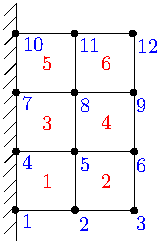
\includegraphics{ensam}
} \hfill
\parbox{0.30\textwidth}{ \begin{footnotesize}
\begin{align*}
ID&=(
\begin{array}{cccccccccccc}
$0$ & $1$ & $2$ & $0$ & $3$ & $4$ & $0$ & $5$ & $6$ & $0$ & $7$ & $8$
\end{array}
) \\
IEN&=\left(
\begin{array}{cccccc}
$1$ & $2$ & $4$ & $5$ & $ 7$ & $ 8$ \\
$2$ & $3$ & $5$ & $6$ & $ 8$ & $ 9$ \\
$5$ & $6$ & $8$ & $9$ & $11$ & $12$ \\
$4$ & $5$ & $7$ & $8$ & $10$ & $11$
\end{array}
\right) \\
LM&=\left(
\begin{array}{cccccc}
$0$ & $1$ & $0$ & $3$ & $ 0$ & $ 5$ \\
$1$ & $2$ & $3$ & $4$ & $ 5$ & $ 6$ \\
$3$ & $4$ & $5$ & $6$ & $ 7$ & $ 8$ \\
$0$ & $3$ & $0$ & $5$ & $ 0$ & $ 7$
\end{array}
\right)
\end{align*}
\end{footnotesize}}
\end{frame}
\newpage
%%%%%%%%%%%%%%%%%%%%%%%%%%%%%%%%%%%%%%%%%%%%%%%%%%%%%%%%%%%%%%%%%%%%%%%%%%%%%%
\begin{frame}
\frametitle{Ensamblaje de las ecuaciones. Ejemplo}
Por ejemplo, para el elemento $3$:
$$
LM(a,3)=\left(
\begin{array}{c}
0 \\
3 \\
5 \\
0
\end{array}
\right) \Rightarrow \qquad
\begin{array}{c}
K_{33} \leftarrow K_{33}+K^e_{22} \\
K_{35} \leftarrow K_{35}+K^e_{23} \\
K_{53} \leftarrow K_{53}+K^e_{32} \\
K_{55} \leftarrow K_{55}+K^e_{33} \\
F_3 \leftarrow F_3 + F^e_2 \\
F_5 \leftarrow F_5 + F^e_3
\end{array}
$$
\end{frame}
%%%%%%%%%%%%%%%%%%%%%%%%%%%%%%%%%%%%%%%%%%%%%%%%%%%%%%%%%%%%%%%%%%%%%%%%%%%%%%
\section{Convergencia}
\begin{frame}
\frametitle{Concepto de convergencia}
\begin{itemize}
\item Al refinar (disminuir el tamaño de los elementos), la solución numérica 
debe aproximarse tanto como se desee a la solución exacta. \pause
\item Consistencia $=$ Complitud $+$ Compatibilidad
\begin{itemize}
\item Complitud: los elementos deben tener la suficiente {\em capacidad
de aproximación} para capturar la solución exacta en límite del proceso
de refinamiento.
\item Compatibilidad: Las funciones de forma deben de ser continuas entre
los elementos \pause
\end{itemize}
\item Estabilidad: se puede interpretar como el requisito que garantiza que la
solución de elementos finitos tiene las mismas propiedades de unicidad que la
solución del modelo matemático que se desea resolver. \pause
\item La complitud es una condición necesaria para la convergencia,
mientras que la relajación de los otros requisitos no excluye la convergencia.
\end{itemize}
\end{frame}
%%%%%%%%%%%%%%%%%%%%%%%%%%%%%%%%%%%%%%%%%%%%%%%%%%%%%%%%%%%%%%%%%%%%%%%%%%%%%%
\begin{frame}
\frametitle{Índice Variacional}
\begin{itemize}
\item El índice variacional $m$ es el orden de la derivada espacial más alta de
$u$ en el funcional de energía $\Pi(u)$.
\item Ejemplo: elasticidad 1D
$$
\Pi(u)=\int_{0}^L \left(\frac{1}{2} u'EAu'-qu \right ) \, dx
\Rightarrow m=1
$$
\item Ejemplo: viga de Euler-Bernoulli
$$
\Pi(u)=\int_{0}^L \left(\frac{1}{2} v''EIv''-qv \right ) \, dx
\Rightarrow m=2
$$
\end{itemize}
\end{frame}
%%%%%%%%%%%%%%%%%%%%%%%%%%%%%%%%%%%%%%%%%%%%%%%%%%%%%%%%%%%%%%%%%%%%%%%%%%%%%%
\begin{frame}
\frametitle{Complitud}
Las funciones de forma deben de representar exactamente todos los polinomios
de grado $\leq m$ en las coordenadas Cartesianas.
\begin{itemize}
\item Este requisito aplica a nivel de elemento y por tanto afecta al conjunto
de funciones de forma del elemento.
\item Elasticidad 2D (m=1)
\begin{equation}
u=\alpha_0 + \alpha_1 x + \alpha_2 y \qquad \qquad
v=\alpha_3 + \alpha_4 x + \alpha_5 \label{ejcomp1}
\end{equation}
Se representan de manera exacta para valores cualesquiera de $\alpha_i$ (movimientos de sólido rígido y campos de deformación constante). La condición de complitud equivale a:
$$
\sum_{a=1}^{n_{en}} N_a = 1
$$
\end{itemize}
\end{frame}
%%%%%%%%%%%%%%%%%%%%%%%%%%%%%%%%%%%%%%%%%%%%%%%%%%%%%%%%%%%%%%%%%%%%%%%%%%%%%%
\begin{frame}
	\frametitle{Complitud}
Por ejemplo $u(x,y)$ debe poder expresarse como:
\begin{equation}
	u(x,y)=\sum_{A=1}^{n_{\rm en}} u^e_A N_A(x,y) \label{ejcomp2}
\end{equation}
siendo $u^e_A$ el valor que toma $u(x,y)$ en el nodo $A$ del elemento $e$:
\begin{equation}
	u^e_A=a_0+a_1 x^e_A + a_2 y^e_A \label{ejcomp3}
\end{equation}

Sustituyendo (\ref{ejcomp3}) en (\ref{ejcomp2}):
\begin{multline}
	u(x,y)=\sum_{A=1}^{n_{\rm en}} (a_0+a_1 x^e_A + a_2 y^e_A) N_A(x,y) \\
	=a_0 \sum_{A=1}^{n_{\rm en}} N_A(x,y)     +
	a_1 \sum_{A=1}^{n_{\rm en}} x^e_A N_A(x,y) +
	a_2 \sum_{A=1}^{n_{\rm en}} y^e_A N_A(x,y)     \label{ejcomp4}
\end{multline}
\end{frame}
%%%%%%%%%%%%%%%%%%%%%%%%%%%%%%%%%%%%%%%%%%%%%%%%%%%%%%%%%%%%%%%%%%%%%%%%%%%%%%
\begin{frame}
Identificando (\ref{ejcomp1}) y (\ref{ejcomp4}) resulta:
\begin{align}
	\sum_{A=1}^{n_{\rm en}} N_A(x,y) &= 1 \label{ejcomp5}  \\
	\sum_{A=1}^{n_{\rm en}} x^e_A N_A(x,y) &= x \label{ejcomp6}  \\
	\sum_{A=1}^{n_{\rm en}} y^e_A N_A(x,y) &= y \label{ejcomp7}
\end{align}
\end{frame}
%%%%%%%%%%%%%%%%%%%%%%%%%%%%%%%%%%%%%%%%%%%%%%%%%%%%%%%%%%%%%%%%%%%%%%%%%%%%%%
\begin{frame}
\frametitle{Compatibilidad}
Las funciones de forma deben ser continuas de clase ${\cal C}^{m-1}$ en las 
fronteras
de elementos adyacentes, y continuas de clase ${\cal C}^{m}$ en el
interior de cada elemento.
\begin{itemize}
\item El requisito de continuidad ${\cal C}^{m-1}$ caracteriza a los
{\em elementos conformes}
\item El requisito de continuidad ${\cal C}^{m}$ caracteriza a las
funciones de {\em energía finita}. Las funciones de forma que lo
satisfacen son funciones cuya derivada $m$-ésima es de cuadrado
integrable: $N(\bm{x}) \in H^m$
\item El requisito de conformidad puede relajarse al límite
asintótico (para $h \rightarrow 0$). La comprobación se realiza mediante
la prueba de la parcela.
\end{itemize}
\begin{center}
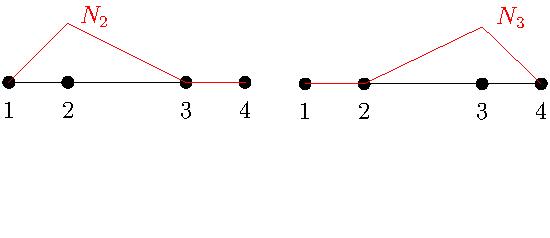
\includegraphics[width=0.7\textwidth]{shape1comp}
\end{center}
\end{frame}
%%%%%%%%%%%%%%%%%%%%%%%%%%%%%%%%%%%%%%%%%%%%%%%%%%%%%%%%%%%%%%%%%%%%%%%%%%%%%%
\begin{frame}
\frametitle{Para ampliar este tema $\ldots$}

\begin{thebibliography}{10}
\beamertemplatebookbibitems
\bibitem{hughes}
{\sc Hughes, T.J.R.}
\newblock {\em The Finite Element Method. Linear Static and Dynamic
Finite Element Analysis.}
\newblock Dover Publications Inc., 2000.

\bibitem{ottosen}
{\sc Ottosen, N. \& Petersson, H.}
\newblock {\em Introduction to the finite element method}.
\newblock Ed. Prentice-Hall, 1992.

\beamertemplatearrowbibitems
\bibitem{felippa}
{\sc Felippa, C.A.}
\newblock {\em  Introduction to Finite Element Methods (ASEN 5007).
Department of Aerospace Engineering Sciences University of Colorado at Boulder.}
\newblock {\tiny \url{http://www.colorado.edu/engineering/CAS/courses.d/IFEM.d/Home.html}}
\end{thebibliography}
\end{frame}
%%%%%%%%%%%%%%%%%%%%%%%%%%%%%%%%%%%%%%%%%%%%%%%%%%%%%%%%%%%%%%%%%%%%%%%%%%%%%%
\end{document}
